 \documentclass{paper}
\usepackage[utf8]{inputenc}

\title{Realidade Virtual}
\author{Sandro Rosevel}
\date{November 2019}

\usepackage{natbib}
\usepackage{graphicx}

\begin{document}



\section{Introdução}
A disciplina de Realidade Virtual ou Realidade Aumentada é voltada as pessoas que possuem interesse em computação gráfica, processamento de imagem ou visão computacional.
Nessa possui foco na aprendizagem da liguagem de GPU CUDA, e em como paralelizar o processamento para que o algoritmo seja executado no maior número de threads possíveis com a mínima dependência entre elas.
\begin{figure}[h!]
\centering
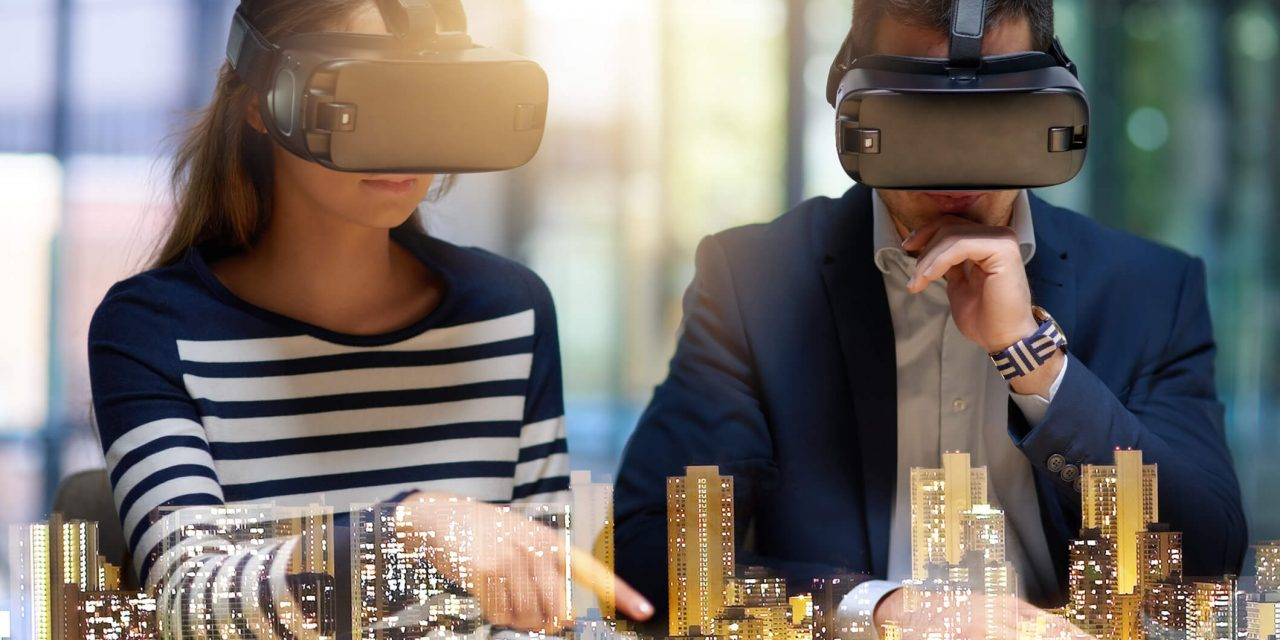
\includegraphics[scale=0.2]{realidade-virtual.jpg}
\caption{realidade virtual}
\label{fig:realidade virtual}
\end{figure}
\section{Relevância}
A utilização de realidade virtual está muito presente no nosso dia-a-dia, e também é utilizada em vários segmentos como, em jogos para entreterimento, simulação e treino de pilotos de avião com a utilização da VR se é possivel economizar dinheiro e tempo com os treinamentos, concepção de projetos para Design, Arquitetura e urbanismo sendo utilizada nesse meio como forma de imersão em espaços, pois muitos usuários ou clientes não conseguem visualizar os conceitos e características de um determinado produto ou serviço\citep{arq2019} e também está ligada a uma área muito importante que é na medicina, sendo utilizada: No tratamentos de dores  foi descoberto que ao desviar a atenção do paciente da dor, pode reduzir cerca de 25 porcento do sofrimento, e por isso a RV foi implantada. No treinamento cirúrgico a VR , por poder recriar várias vezes uma cena ficticia e realista ao mesmo tempo, é perfeita para o treinamento de profissionais da saúde como: médicos, enfermeiros e cuidadores de pacientes. A VR já é aplicada em procedimentos como cirurgias e trabalhos de parto para o treinamento de novos médicos por ter funcionalidades de poderem repetir operações quantas vezes forem necessárias, sem riscos aos pacientes. E no tratamento de transtornos e fobias, O uso da VR na pscicologia vem como mais uma técnica para complementar o tratamento de diversos transtornos e fobias, tais como: transtorno do pânico, medo de injeções e agulhas, aerofobia transtorno obsessivo compulsivo, ansiedade e muitos outros.\citep{med2019} \citep{fob2019}
\section{Relação com outras disciplinas}
A disciplina possui relação com outras duas disciplinas apresentadas no perfil curricular que são:IF681 - Interfaces usuario-maquina
IF687- Introdução a multimidia, que são ofertadas no quarto e quinto periodo.


\bibliographystyle{plain}
\bibliography{svrs2}
\end{document}
